\section{Resultados} \label{sec:resultados}

\subsection{Rotações}

    \begin{figure}[H]
    \centering\hfill
    \begin{subfigure}{0.4\textwidth}
        \centering
        
\includegraphics[width=0.9\textwidth]{rotacoes/16_alp_viz.png}
        \caption{~\texttt{vizinho}.}
    \end{subfigure}%
    \hfill%
    \begin{subfigure}{0.4\textwidth}
        \centering
        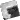
\includegraphics[width=0.9\textwidth]{rotacoes/16_alp_bil.png}
        \caption{~\texttt{bilinear}.}
    \end{subfigure}\hfill
    \\[8pt]\hfill
    \begin{subfigure}{0.4\textwidth}
        \centering
        \includegraphics[width=0.9\textwidth]{rotacoes/16_alp_bic.png}
        \caption{~\texttt{bicubica}.}
    \end{subfigure}%
    \hfill%
    \begin{subfigure}{0.4\textwidth}
        \centering
        \includegraphics[width=0.9\textwidth]{rotacoes/16_alp_lag.png}
        \caption{~\texttt{lagrange}.}
    \end{subfigure}\hfill

    \caption{Rotação de 15\textdegree{} no plano da imagem aplicada em \texttt{house16.png} ($16 \times 16$).}
    \label{fig:house16:alp}
\end{figure}

    Na \cref{fig:rot:house64}, podemos ver com clareza a diferença entre os métodos. Nas interpolações bilinear e bicúbica, a imagem resultante aparece com um pequeno borramento. Esse efeito é bem mais fraco com polinômios de Lagrange.

    Para o aproximação por vizinho mais próximo, a figura fica com um serrilhado bem presente, principalmente nas bordas. Isso aparece inclusive em imagens grandes, como na \cref{fig:rot:house}. Além desse método, quase não existem diferenças visuais para as imagens de $512 \times 512$.

    \begin{figure}[H]
    \centering
    \begin{subfigure}{0.3\textwidth}
        \centering
        \includegraphics[width=0.8\textwidth]{rotacoes/64_alp_viz.png}
        \caption{~\texttt{vizinho}.}
    \end{subfigure}%
    \hspace{8pt}%
    \begin{subfigure}{0.3\textwidth}
        \centering
        \includegraphics[width=0.8\textwidth]{rotacoes/64_alp_bil.png}
        \caption{~\texttt{bilinear}.}
    \end{subfigure}
    \\[8pt]
    \begin{subfigure}{0.3\textwidth}
        \centering
        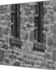
\includegraphics[width=0.8\textwidth]{rotacoes/64_alp_bic.png}
        \caption{~\texttt{bicubica}.}
    \end{subfigure}%
    \hspace{8pt}%
    \begin{subfigure}{0.3\textwidth}
        \centering
        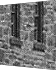
\includegraphics[width=0.8\textwidth]{rotacoes/64_alp_lag.png}
        \caption{~\texttt{lagrange}.}
    \end{subfigure}

    \caption{Rotação de -30\textdegree{} no plano da imagem aplicada em \texttt{house16.png} ($64 \times 64$).}
    \label{fig:rot:house64}
\end{figure}

    \begin{figure}[H]
    \centering
    \begin{subfigure}{0.33\textwidth}
        \centering
        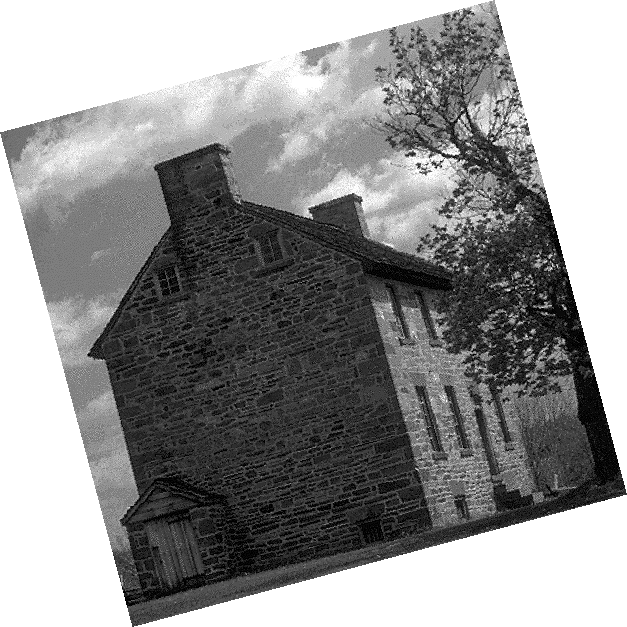
\includegraphics[width=0.9\textwidth]{rotacoes/house_alp_viz.png}
        \caption{~\texttt{vizinho}.}
    \end{subfigure}%
    \hspace{8pt}
    \begin{subfigure}{0.33\textwidth}
        \centering
        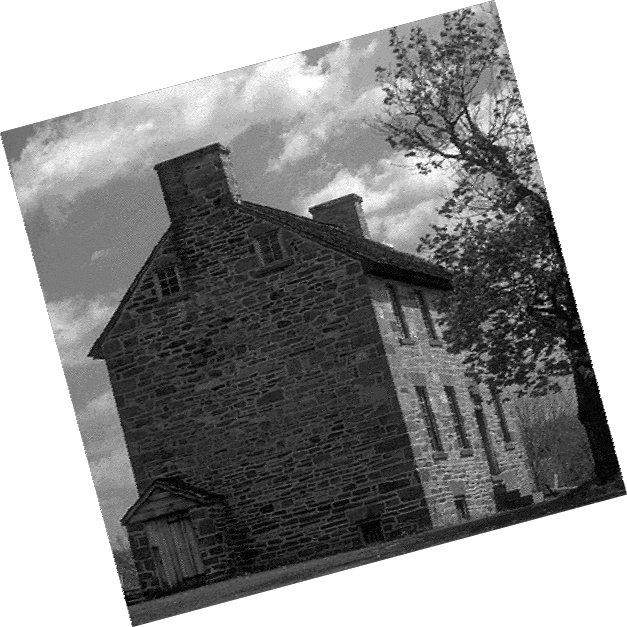
\includegraphics[width=0.9\textwidth]{rotacoes/house_alp_bil.png}
        \caption{~\texttt{bilinear}.}
    \end{subfigure}
    \\[8pt]
    \begin{subfigure}{0.33\textwidth}
        \centering
        \includegraphics[width=0.9\textwidth]{rotacoes/house_alp_bic.png}
        \caption{~\texttt{bicubica}.}
    \end{subfigure}%
    \hspace{8pt}%
    \begin{subfigure}{0.33\textwidth}
        \centering
        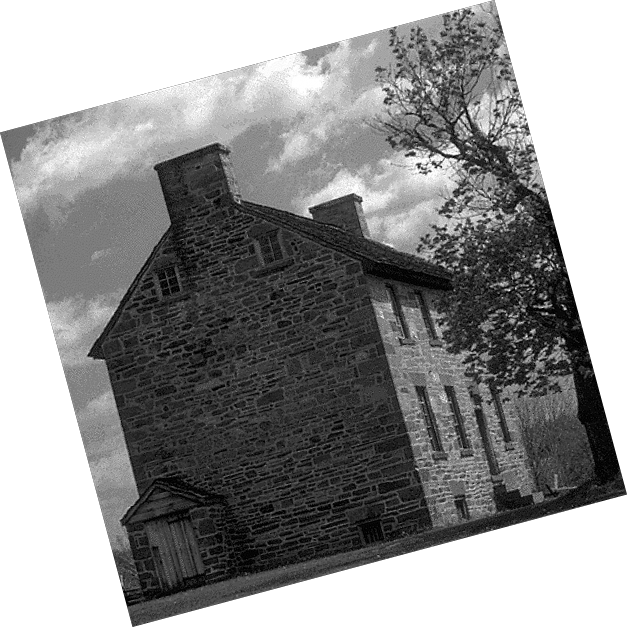
\includegraphics[width=0.9\textwidth]{rotacoes/house_alp_lag.png}
        \caption{~\texttt{lagrange}.}
    \end{subfigure}

    \caption{Rotação de 15\textdegree{} no plano da imagem aplicada em \texttt{house.png} ($512 \times 512$).}
    \label{fig:rot:house}
\end{figure}

\subsection{Escalonamento}

    \begin{figure}[H]
    \centering
    \begin{subfigure}{0.3\textwidth}
        \centering
        \includegraphics[width=0.9\textwidth]{escala/city_13_viz.png}
        \caption{~\texttt{vizinho}.}
    \end{subfigure}%
    \hspace{8pt}
    \begin{subfigure}{0.3\textwidth}
        \centering
        \includegraphics[width=0.9\textwidth]{escala/city_13_bil.png}
        \caption{~\texttt{bilinear}.}
    \end{subfigure}
    \\[8pt]
    \begin{subfigure}{0.3\textwidth}
        \centering
        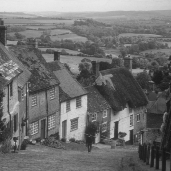
\includegraphics[width=0.9\textwidth]{escala/city_13_bic.png}
        \caption{~\texttt{bicubica}.}
    \end{subfigure}%
    \hspace{8pt}%
    \begin{subfigure}{0.3\textwidth}
        \centering
        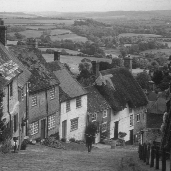
\includegraphics[width=0.9\textwidth]{escala/city_13_lag.png}
        \caption{~\texttt{lagrange}.}
    \end{subfigure}

    \caption{Escalonamento com $S_x = S_y = 1/3$ aplicado em \texttt{city.png} ($512 \times 512$).}
    \label{fig:esc:13}
\end{figure}

    \begin{figure}[H]
    \centering
    \begin{subfigure}{0.3\textwidth}
        \centering
        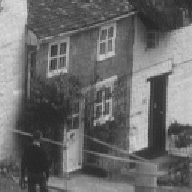
\includegraphics[width=0.9\textwidth]{escala/128_15_viz.png}
        \caption{~\texttt{vizinho}.}
    \end{subfigure}%
    \hspace{8pt}
    \begin{subfigure}{0.3\textwidth}
        \centering
        \includegraphics[width=0.9\textwidth]{escala/128_15_bil.png}
        \caption{~\texttt{bilinear}.}
        \label{fig:esc:15:bil}
    \end{subfigure}
    \\[8pt]
    \begin{subfigure}{0.3\textwidth}
        \centering
        \includegraphics[width=0.9\textwidth]{escala/128_15_bic.png}
        \caption{~\texttt{bicubica}.}
    \end{subfigure}%
    \hspace{8pt}%
    \begin{subfigure}{0.3\textwidth}
        \centering
        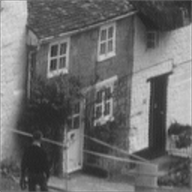
\includegraphics[width=0.9\textwidth]{escala/128_15_lag.png}
        \caption{~\texttt{lagrange}.}
    \end{subfigure}

    \caption{Escalonamento com $S_x = S_y = 1.5$ aplicado em \texttt{city128.png} ($128 \times 128$).}
    \label{fig:esc:15}
\end{figure}

    No caso da mudança de escala, podemos ver que a bicúbica tem os melhores resultados na redução das dimensões, que acontece na \cref{fig:esc:13}. No entanto, para ampliação da imagem (\cref{fig:esc:15}), o borramento da imagem é muito forte, fazendo com que o método por polinômios de Lagrange tenha resultados melhores. Isso também acontece na \cref{fig:esc:86}, por ser muito pequeno o resultado.

    Tanto na ampliação (\ref{fig:esc:15:bil}), quanto na redução (\ref{fig:esc:13:bil}), o método bilinear gerou artefatos muito presentes nas bordas dos objetos. No entanto, isso pode ser devido à implementação e não necessariamente ao método. Um efeito similar aconteceu usando os vizinhos mais próximos.

    \begin{figure}[H]
    \centering
    \begin{subfigure}{0.33\textwidth}
        \centering
        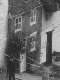
\includegraphics[width=0.8\textwidth]{escala/128_86_viz.png}
        \caption{~\texttt{vizinho}.}
    \end{subfigure}%
    \hspace{8pt}
    \begin{subfigure}{0.33\textwidth}
        \centering
        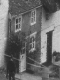
\includegraphics[width=0.8\textwidth]{escala/128_86_bil.png}
        \caption{~\texttt{bilinear}.}
    \end{subfigure}
    \\[8pt]
    \begin{subfigure}{0.33\textwidth}
        \centering
        \includegraphics[width=0.8\textwidth]{escala/128_86_bic.png}
        \caption{~\texttt{bicubica}.}
    \end{subfigure}%
    \hspace{8pt}%
    \begin{subfigure}{0.33\textwidth}
        \centering
        \includegraphics[width=0.8\textwidth]{escala/128_86_lag.png}
        \caption{~\texttt{lagrange}.}
    \end{subfigure}

    \caption{Redimensionamento para $80 \times 60$ aplicado em \texttt{city128.png} ($128 \times 128$).}
    \label{fig:esc:86}
\end{figure}

\subsection{Reconstrução}

    \begin{figure}[H]
        \centering
        \includegraphics[width=0.27\textwidth]{../imagens/baboon128.png}
        \caption{\texttt{baboon128.png} ($128 \times 128$).}
        \label{fig:baboon128}
    \end{figure}

    Tentando aplicar uma transformação simples, de escala (\cref{fig:rec:x2}) ou de rotação (\cref{fig:rec:45}), seguida da sua inversa podemos ver que as interpolações bilinear e bicúbica causam um efeito de \textit{blur} muito presente. Para valores racionais, como $S_x = S_y = 1.37$, pode ser que o arredondamento acabe causando artefatos maiores no método dos vizinhos mais próximos.

    \begin{figure}[H]
    \centering
    \begin{subfigure}{0.3\textwidth}
        \centering
        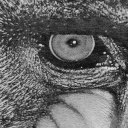
\includegraphics[width=0.9\textwidth]{reconstrucao/baboon_x2_viz.png}
        \caption{~\texttt{vizinho}.}
    \end{subfigure}%
    \hspace{8pt}
    \begin{subfigure}{0.3\textwidth}
        \centering
        \includegraphics[width=0.9\textwidth]{reconstrucao/baboon_x2_bil.png}
        \caption{~\texttt{bilinear}.}
    \end{subfigure}
    \\[8pt]
    \begin{subfigure}{0.3\textwidth}
        \centering
        \includegraphics[width=0.9\textwidth]{reconstrucao/baboon_x2_bic.png}
        \caption{~\texttt{bicubica}.}
    \end{subfigure}%
    \hspace{8pt}%
    \begin{subfigure}{0.3\textwidth}
        \centering
        \includegraphics[width=0.9\textwidth]{reconstrucao/baboon_x2_lag.png}
        \caption{~\texttt{lagrange}.}
    \end{subfigure}

    \caption{Escalonamento por um fator 2 seguido de outro escalonamento de fator 1/2 em \texttt{baboon128.png}, usando o mesmo método em cada caso.}
    \label{fig:rec:x2}
\end{figure}

    \begin{figure}[H]
    \centering
    \begin{subfigure}{0.33\textwidth}
        \centering
        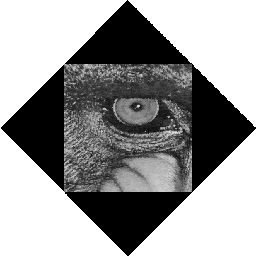
\includegraphics[width=0.95\textwidth]{reconstrucao/baboon_45_viz.png}
        \caption{~\texttt{vizinho}.}
    \end{subfigure}%
    \hspace{8pt}
    \begin{subfigure}{0.33\textwidth}
        \centering
        \includegraphics[width=0.95\textwidth]{reconstrucao/baboon_45_bil.png}
        \caption{~\texttt{bilinear}.}
    \end{subfigure}
    \\[8pt]
    \begin{subfigure}{0.33\textwidth}
        \centering
        \includegraphics[width=0.95\textwidth]{reconstrucao/baboon_45_bic.png}
        \caption{~\texttt{bicubica}.}
    \end{subfigure}%
    \hspace{8pt}%
    \begin{subfigure}{0.33\textwidth}
        \centering
        \includegraphics[width=0.95\textwidth]{reconstrucao/baboon_45_lag.png}
        \caption{~\texttt{lagrange}.}
    \end{subfigure}

    \caption{Rotação de 45\textdegree{} (com borda preta) seguida de outra rotação de -45\textdegree{} no plano da imagem em \texttt{baboon128.png}, usando o mesmo método em cada caso.}
    \label{fig:rec:x2}
\end{figure}

\subsection{Tempo de Execução}

    \begin{figure}[H]
        \centering
        \includegraphics[width=0.3\textwidth]{../imagens/among.png}
        \caption{\texttt{among.png} ($2000 \times 1544$).}
        \label{fig:among}
    \end{figure}
